\chapter[Cooling, Feedback, and Ionizing Sources]{One Zone Cooling, Feedback, and Ionizing Source Closure}
\label{ch:cooling-feedback-reionization}

% Generated by Cooling_Feedback_Reionization_Verification.py
\newcommand{\CFRAtomicVelocity}{16.727527}
\newcommand{\CFRPairZoom}{53}
\newcommand{\CFRPairControl}{52}
\newcommand{\CFRMassResidual}{1.807e-15}
\newcommand{\CFRZoomTotalStarMin}{0.960484}
\newcommand{\CFRZoomTotalStarMedian}{0.962352}
\newcommand{\CFRZoomTotalStarMax}{0.966885}
\newcommand{\CFRControlTotalStarMin}{0.960151}
\newcommand{\CFRControlTotalStarMedian}{0.962225}
\newcommand{\CFRControlTotalStarMax}{0.966525}
\newcommand{\CFRZoomDwarfStarMin}{0.461458}
\newcommand{\CFRZoomDwarfStarMedian}{0.549254}
\newcommand{\CFRZoomDwarfStarMax}{0.606955}
\newcommand{\CFRControlDwarfStarMin}{0.482247}
\newcommand{\CFRControlDwarfStarMedian}{0.597254}
\newcommand{\CFRControlDwarfStarMax}{0.652880}
\newcommand{\CFRZoomDwarfSFRMin}{0.441567}
\newcommand{\CFRZoomDwarfSFRMedian}{0.517358}
\newcommand{\CFRZoomDwarfSFRMax}{0.616550}
\newcommand{\CFRControlDwarfSFRMin}{0.432337}
\newcommand{\CFRControlDwarfSFRMedian}{0.508604}
\newcommand{\CFRControlDwarfSFRMax}{0.619121}
\newcommand{\CFRIonMin}{0.433826}
\newcommand{\CFRIonMedian}{0.520843}
\newcommand{\CFRIonMax}{0.639050}
\newcommand{\CFRBoostMin}{1.564824}
\newcommand{\CFRBoostMedian}{1.919965}
\newcommand{\CFRBoostMax}{2.305070}
\newcommand{\CFRPriorPenalty}{2.921558}
\newcommand{\CFROrderedZoom}{17}
\newcommand{\CFROrderedControl}{18}
\newcommand{\CFRMaxOrderedStar}{0.966845}
\newcommand{\CFRPass}{20}
\newcommand{\CFRFail}{0}


\section{Scope and objective}

The scale covariant refinement model now has a fixed collisionless transfer function, primary and late time observable calculations, nonlinear particle evolution, paired halo catalogues, and broad baryonic response envelopes.  The unresolved physical interface is the conversion of halo growth into gas, stars, outflows, and ionizing sources.

This chapter introduces a mass conserving one zone regulator.  It is applied to the cold and refinement halo histories with exactly the same cooling and feedback parameters.  No dark sector parameter is retuned.  The calculation has two purposes:
\begin{enumerate}
\item replace the previous static baryonic response map by a time dependent gas budget with explicit inflow, cooling, star formation, recycling, and outflow;
\item propagate the same response law into the high redshift halo mass functions and measure the remaining ionizing emissivity burden.
\end{enumerate}

The principal result is
\begin{equation}
\boxed{
\begin{aligned}
\text{matched total stellar budget} &\simeq 0.96\times\text{cold},\\
\text{near cutoff stellar mass and SFR} &\simeq 0.4\text{--}0.65\times\text{cold},\\
\text{ionizing source at }z=7.4 &\simeq 0.43\text{--}0.64\times\text{cold},\\
\text{required source enhancement} &\simeq 1.56\text{--}2.31.
\end{aligned}}
\label{eq:cfr-principal-result}
\end{equation}

The calculation is a controlled one zone closure.  It is not a hydrodynamic simulation and does not resolve a multiphase interstellar medium.

\section{Virial temperature and the atomic cooling scale}

For mean molecular weight $\mu$, define the virial temperature from the halo speed $V$ by
\begin{equation}
T_{\rm vir}(V)
=
\frac{\mu m_pV^2}{2k_B}.
\label{eq:cfr-virial-temperature}
\end{equation}
With $\mu=0.59$,
\begin{equation}
T_{\rm vir}
=
35.74\ {\rm K}
\left(\frac{V}{1\ {\rm km\,s^{-1}}}\right)^2.
\label{eq:cfr-temperature-speed}
\end{equation}
The declared atomic threshold $T_{\rm atom}=10^4\ {\rm K}$ therefore corresponds to
\begin{equation}
\boxed{
V_{\rm atom}=\CFRAtomicVelocity\ {\rm km\,s^{-1}}.
}
\label{eq:cfr-atomic-speed}
\end{equation}

The smooth atomic cooling gate is
\begin{equation}
C_{\rm atom}(V)
=
\left[
1+
\left(
\frac{T_{\rm atom}}{T_{\rm vir}(V)}
\right)^{n_{\rm atom}}
\right]^{-1}.
\label{eq:cfr-atomic-gate}
\end{equation}
After the calibrated reionization midpoint, the photoheating gate is
\begin{equation}
C_{\rm ph}(V)
=
\left[
1+
\left(
\frac{V_{\rm ph}}{V}
\right)^4
\right]^{-1}.
\label{eq:cfr-photo-gate}
\end{equation}
Before reionization, $C_{\rm ph}=1$.

Energy driven outflow is represented by the mass loading
\begin{equation}
\eta_w(V)
=
\left(
\frac{V_{\rm fb}}{V}
\right)^\beta.
\label{eq:cfr-mass-loading}
\end{equation}
This response is common to both dark matter branches.

\section{Mass conserving gas regulator}

Let $M_h(a)$ be one halo growth history.  Define gas, long lived stars, and expelled material by
\begin{equation}
M_g(a),\qquad M_\star(a),\qquad M_{\rm out}(a).
\end{equation}
Use the stellar return fraction $R$ and a dynamical time
\begin{equation}
t_{\rm dyn}=\xi H^{-1},
\qquad
\xi=0.1.
\label{eq:cfr-dynamical-time}
\end{equation}
The star formation rate before recycling is
\begin{equation}
\psi
=
\frac{\epsilon_{\rm ff}}{t_{\rm dyn}}
C_{\rm atom}C_{\rm ph}M_g.
\label{eq:cfr-star-formation-rate}
\end{equation}
Using $a$ as the independent variable, the regulator is
\begin{align}
\frac{dM_g}{da}
&=
f_b\frac{dM_h}{da}
-
\frac{\epsilon_{\rm ff}C_{\rm atom}C_{\rm ph}}{\xi a}
(1-R+\eta_w)M_g,
\label{eq:cfr-gas-equation}
\\
\frac{dM_\star}{da}
&=
\frac{\epsilon_{\rm ff}C_{\rm atom}C_{\rm ph}}{\xi a}
(1-R)M_g,
\label{eq:cfr-star-equation}
\\
\frac{dM_{\rm out}}{da}
&=
\frac{\epsilon_{\rm ff}C_{\rm atom}C_{\rm ph}}{\xi a}
\eta_wM_g.
\label{eq:cfr-outflow-equation}
\end{align}

\begin{theorem}[Exact baryonic mass budget]
For every nondecreasing halo history,
\begin{equation}
\frac{d}{da}
\left(
M_g+M_\star+M_{\rm out}-f_bM_h
\right)
=0.
\label{eq:cfr-budget-derivative}
\end{equation}
If the initial state satisfies $M_g=f_bM_h$ and $M_\star=M_{\rm out}=0$, then
\begin{equation}
\boxed{
M_g(a)+M_\star(a)+M_{\rm out}(a)=f_bM_h(a)
}
\label{eq:cfr-exact-budget}
\end{equation}
for all later $a$.
\end{theorem}

\begin{proof}
Add equations \eqref{eq:cfr-gas-equation} through \eqref{eq:cfr-outflow-equation}.  The cooling, star formation, recycling, and outflow terms cancel exactly.  Only the baryonic halo inflow remains.
\end{proof}

The numerical update integrates the linear gas equation exactly over each scale factor interval after freezing the midpoint coefficients.  The removed gas is divided between stars and outflow in the exact ratio $(1-R):\eta_w$.  The largest recorded relative budget residual is
\begin{equation}
\boxed{\CFRMassResidual.}
\label{eq:cfr-budget-residual}
\end{equation}

\section{Feedback amplification}

In the slowly varying equilibrium limit, equation \eqref{eq:cfr-gas-equation} gives
\begin{equation}
\dot M_{\star,\rm eq}
=
f_b\dot M_h
C_{\rm cool}
\frac{1-R}{1-R+\eta_w},
\qquad
C_{\rm cool}=C_{\rm atom}C_{\rm ph}.
\label{eq:cfr-equilibrium-sfr}
\end{equation}
For a matched pair,
\begin{equation}
\frac{\dot M_{\star,R}}{\dot M_{\star,C}}
=
\frac{\dot M_{h,R}}{\dot M_{h,C}}
\frac{C_R}{C_C}
\frac{1-R+\eta_C}{1-R+\eta_R}.
\label{eq:cfr-feedback-ratio}
\end{equation}
If $V_R\leq V_C$, then $C_R\leq C_C$ in the atomic and photoheating regime and $\eta_R\geq\eta_C$.  Therefore
\begin{equation}
\boxed{
\frac{\dot M_{\star,R}}{\dot M_{\star,C}}
\leq
\frac{\dot M_{h,R}}{\dot M_{h,C}}.
}
\label{eq:cfr-feedback-amplification}
\end{equation}
A modest gravitational reduction can therefore become a larger luminous reduction.

Figure~\ref{fig:cfr-feedback-efficiency} shows the equilibrium retained star fraction.  The atomic threshold and energy driven outflow act in the same direction for low speed halos.

\begin{figure}[htbp]
\centering
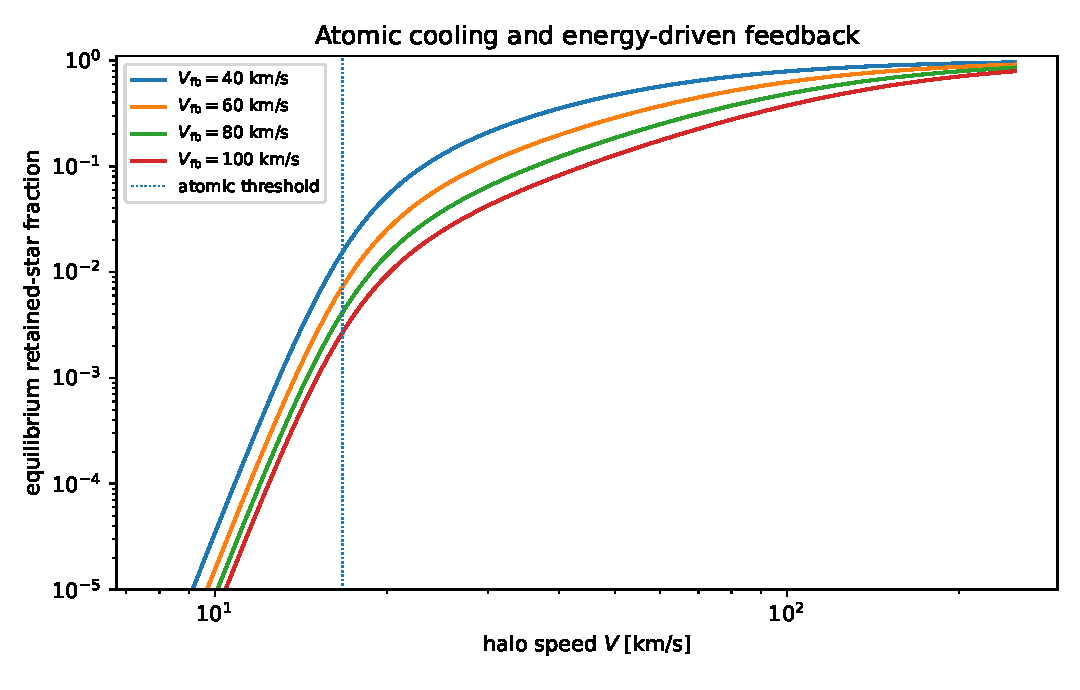
\includegraphics[width=.82\linewidth]{figures/cfr/04_feedback_efficiency.pdf}
\caption{Equilibrium retained star fraction for the declared feedback speeds.  The atomic cooling threshold is fixed by equation \eqref{eq:cfr-atomic-speed}.}
\label{fig:cfr-feedback-efficiency}
\end{figure}

\section{Matched assembly histories}

The paired halo catalogues provide final mass and speed together with the fraction of final particles already contained in the largest progenitor at $a=0.5$.  For each branch, the controlled interpolation is
\begin{equation}
M_h(a)=M_{h,1}a^s,
\qquad
s=
\frac{\log f_{1/2}}{\log(1/2)}.
\label{eq:cfr-growth-history}
\end{equation}
The speed history is normalized to the measured final value,
\begin{equation}
V(a)
=
V_1
\left(
\frac{M_h(a)}{M_{h,1}}
\right)^{1/3}
E(a)^{1/3}.
\label{eq:cfr-speed-history}
\end{equation}

The main matched sample contains $\CFRPairZoom$ pairs.  The time control contains $\CFRPairControl$ pairs.  The response grid contains
\begin{equation}
3\times4\times3\times4\times3=432
\label{eq:cfr-parameter-count}
\end{equation}
common baryonic parameter choices:
\begin{align}
\epsilon_{\rm ff}&\in\{0.005,0.01,0.02\},\\
V_{\rm fb}&\in\{40,60,80,100\}\ {\rm km\,s^{-1}},\\
\beta&\in\{1.5,2,3\},\\
V_{\rm ph}&\in\{15,20,25,30\}\ {\rm km\,s^{-1}},\\
n_{\rm atom}&\in\{2,4,8\}.
\end{align}

For the representative choice
\begin{equation}
(\epsilon_{\rm ff},V_{\rm fb},\beta,V_{\rm ph},n_{\rm atom})
=(0.01,80,2,20,4),
\label{eq:cfr-representative-parameters}
\end{equation}
the aggregate stellar and current star formation ratios approach the final halo mass ratio while retaining a larger early difference.

\begin{figure}[htbp]
\centering
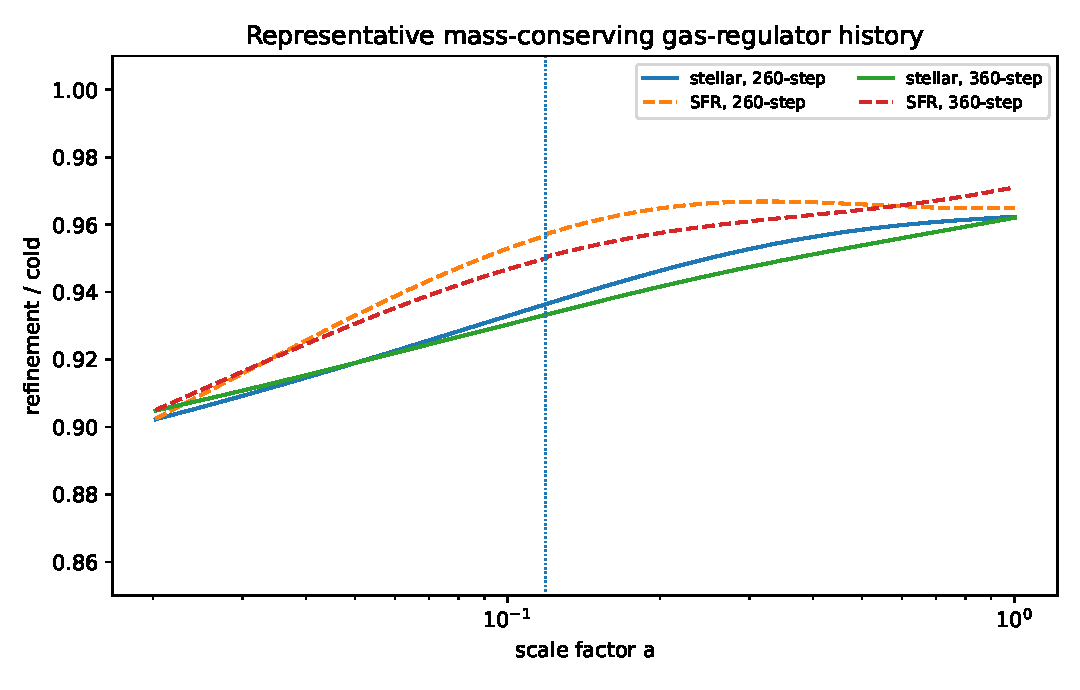
\includegraphics[width=.84\linewidth]{figures/cfr/01_regulator_history.pdf}
\caption{Representative matched sample regulator history.  The vertical marker is the calibrated reionization midpoint.}
\label{fig:cfr-regulator-history}
\end{figure}

\section{Resolved matched baryonic response}

Across the full parameter grid, the matched total stellar ratio is
\begin{equation}
\boxed{
\CFRZoomTotalStarMin
\leq
\frac{M_{\star,R}^{\rm matched}}{M_{\star,C}^{\rm matched}}
\leq
\CFRZoomTotalStarMax
}
\label{eq:cfr-total-star-zoom}
\end{equation}
in the main sample and
\begin{equation}
\boxed{
\CFRControlTotalStarMin
\leq
\frac{M_{\star,R}^{\rm matched}}{M_{\star,C}^{\rm matched}}
\leq
\CFRControlTotalStarMax
}
\label{eq:cfr-total-star-control}
\end{equation}
in the time control.  The medians are $\CFRZoomTotalStarMedian$ and $\CFRControlTotalStarMedian$.

The near cutoff response is much stronger.  For matched cold halos with
\begin{equation}
M_C\leq3\times10^{10}\ M_\odot/h,
\end{equation}
the stellar mass envelopes are
\begin{equation}
\boxed{
\CFRZoomDwarfStarMin
\leq
\operatorname{median}\frac{M_{\star,R}}{M_{\star,C}}
\leq
\CFRZoomDwarfStarMax
}
\label{eq:cfr-dwarf-star-zoom}
\end{equation}
and
\begin{equation}
\boxed{
\CFRControlDwarfStarMin
\leq
\operatorname{median}\frac{M_{\star,R}}{M_{\star,C}}
\leq
\CFRControlDwarfStarMax.
}
\label{eq:cfr-dwarf-star-control}
\end{equation}

The corresponding present star formation rate envelopes are
\begin{equation}
\boxed{
\CFRZoomDwarfSFRMin
\leq
\operatorname{median}\frac{\dot M_{\star,R}}{\dot M_{\star,C}}
\leq
\CFRZoomDwarfSFRMax
}
\label{eq:cfr-dwarf-sfr-zoom}
\end{equation}
and
\begin{equation}
\boxed{
\CFRControlDwarfSFRMin
\leq
\operatorname{median}\frac{\dot M_{\star,R}}{\dot M_{\star,C}}
\leq
\CFRControlDwarfSFRMax.
}
\label{eq:cfr-dwarf-sfr-control}
\end{equation}

Thus the matched total budget is nearly cold like, while the near cutoff stellar mass and current activity are lower by approximately forty percent to sixty percent.

\begin{figure}[htbp]
\centering
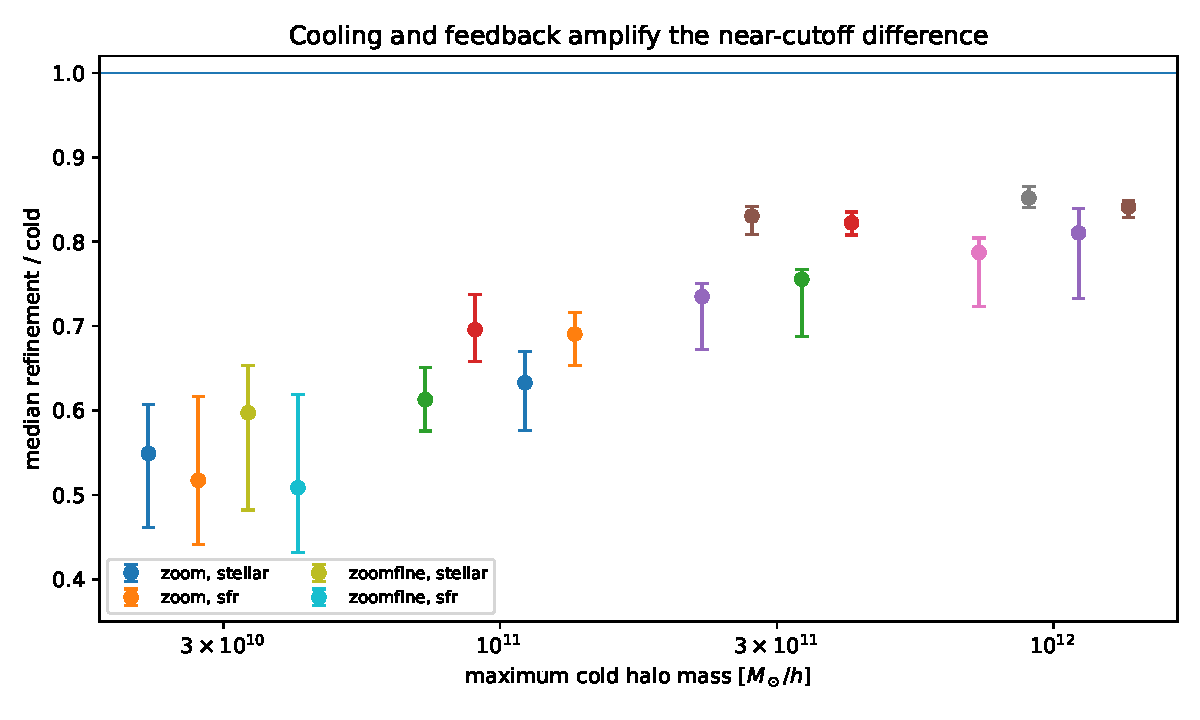
\includegraphics[width=.88\linewidth]{figures/cfr/02_dwarf_response_envelopes.pdf}
\caption{Median stellar mass and present star formation response envelopes as the maximum matched cold halo mass is increased.}
\label{fig:cfr-dwarf-envelopes}
\end{figure}

\section{Ordered source theorem and the assembly boundary}

A strict subset of matched pairs satisfies, throughout the declared history,
\begin{equation}
M_R(a)\leq M_C(a),
\qquad
M_R'(a)\leq M_C'(a),
\qquad
V_R(a)\leq V_C(a).
\label{eq:cfr-source-order}
\end{equation}
There are $\CFROrderedZoom$ such pairs in the main sample and $\CFROrderedControl$ in the time control.

For these source ordered histories, the common regulator produces no integrated stellar ordering violation anywhere in the $432$ point response grid.  The largest ratio is
\begin{equation}
\boxed{
\max
\frac{M_{\star,R}}{M_{\star,C}}
=
\CFRMaxOrderedStar<1.
}
\label{eq:cfr-max-ordered-star}
\end{equation}

Pairs whose assembly histories cross need not obey a pointwise comparison theorem.  Their integrated stellar ratio can depend on when gas entered the halo, not only on the final mass and speed.  This is an important boundary.  A final halo deficit does not by itself determine a unique stellar history.

\section{Feedback weighted ionizing emissivity}

At redshift $z$, let $dn_X/d\log M$ be the cold or refinement halo mass function.  The common equilibrium ionizing source proxy is
\begin{equation}
\dot n_{\gamma,X}(z)
\propto
\int_{M_{\rm atom}(z)}^\infty
M
\epsilon_{\rm src}(M,z)
\frac{dn_X}{d\log M}
\,d\log M,
\label{eq:cfr-ionizing-source}
\end{equation}
where
\begin{equation}
\epsilon_{\rm src}
=
C_{\rm atom}C_{\rm ph}
\frac{1-R}{1-R+\eta_w}.
\label{eq:cfr-source-efficiency}
\end{equation}
The atomic cooling threshold is
\begin{equation}
M_{\rm atom}(z)
=
10^8M_\odot
\left(
\frac{1+z}{10}
\right)^{-3/2}.
\label{eq:cfr-atomic-mass}
\end{equation}
Common photon production and escape factors cancel from the refinement to cold ratio.

At $z=7.4$, including the declared photoheating response,
\begin{equation}
\boxed{
\CFRIonMin
\leq
\frac{\dot n_{\gamma,R}}{\dot n_{\gamma,C}}
\leq
\CFRIonMax,
\qquad
\operatorname{median}=\CFRIonMedian.
}
\label{eq:cfr-ionizing-envelope}
\end{equation}
The required common source efficiency enhancement is
\begin{equation}
\boxed{
\CFRBoostMin
\leq
\frac{\epsilon_{\gamma,R}}{\epsilon_{\gamma,C}}
\leq
\CFRBoostMax,
\qquad
\operatorname{median}=\CFRBoostMedian.
}
\label{eq:cfr-ionizing-boost}
\end{equation}

The earlier unweighted collapsed fraction penalty at the same redshift was $\CFRPriorPenalty$.  Weighting the source toward halos that cool and retain gas reduces the median burden to $\CFRBoostMedian$, but does not remove it.

\begin{figure}[htbp]
\centering
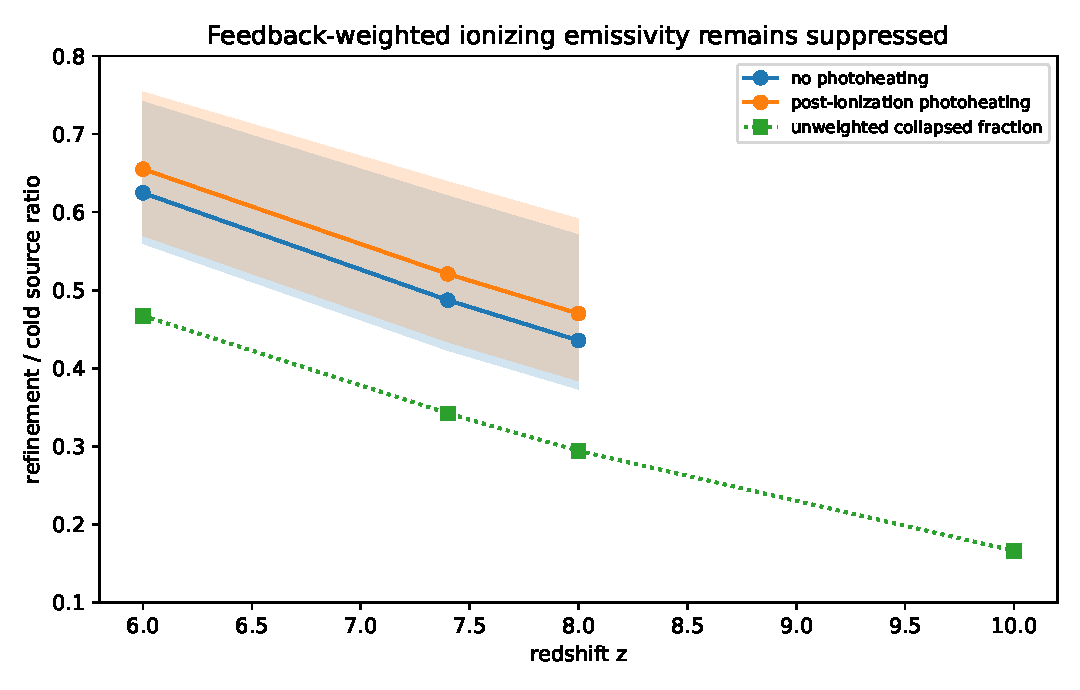
\includegraphics[width=.82\linewidth]{figures/cfr/03_ionizing_emissivity.pdf}
\caption{Feedback weighted ionizing emissivity.  The square markers show the earlier unweighted collapsed fraction ratio.}
\label{fig:cfr-ionizing-emissivity}
\end{figure}

The redshift dependence is
\begin{center}
\begin{tabular}{lccc}
\toprule
redshift & minimum source ratio & median source ratio & maximum source ratio\\
\midrule
$6.0$ & $0.5699$ & $0.6552$ & $0.7539$\\
$7.4$ & $0.4338$ & $0.5208$ & $0.6390$\\
$8.0$ & $0.3841$ & $0.4701$ & $0.5915$\\
\bottomrule
\end{tabular}
\end{center}
The reionization pressure therefore grows rapidly toward earlier epochs.

\section{Scientific interpretation}

The fixed parameter pattern is now more specific:
\begin{equation}
\boxed{
\begin{aligned}
\text{massive matched systems:}&\quad \text{nearly cold like integrated baryon budget},\\
\text{near cutoff systems:}&\quad \text{lower stellar mass and lower present star formation},\\
\text{early ionizing sources:}&\quad \text{suppressed by roughly thirty five percent to sixty percent},\\
\text{reionization:}&\quad \text{requires a source efficiency enhancement of order two}.
\end{aligned}}
\label{eq:cfr-physical-pattern}
\end{equation}

This sharpens the observational hierarchy.  Total stellar mass density is not the strongest discriminator.  Dwarf activity, early galaxies, escape fraction requirements, and the timing of reionization retain more information about the refinement cutoff.

\section{Verification}

The deterministic audit records
\begin{equation}
\boxed{
\CFRPass\ {\rm PASS},
\qquad
\CFRFail\ {\rm FAIL}.
}
\label{eq:cfr-pass-count}
\end{equation}
The checks cover the atomic threshold, the complete parameter grid, sample size, exact mass conservation, positivity, matched total suppression, dwarf stellar and star formation envelopes, source ordered histories, ionizing source suppression, and time control agreement.

\section{Claim boundary}

This chapter establishes an exact mass budget and controlled response calculations within the declared one zone model.  It does not establish:
\begin{itemize}
\item a resolved Euler or magnetohydrodynamic simulation;
\item molecular cooling, metal line cooling, dust, or a multiphase interstellar medium;
\item calibrated stellar populations, supernova yields, or escape fractions;
\item radiation transport or a predicted reionization optical depth;
\item converged subhalos, satellite disruption, or disk shocking;
\item a survey likelihood or empirical correctness;
\item a microscopic derivation of the refinement production scale and coupling.
\end{itemize}

The strongest retained result is not a precision galaxy prediction.  It is a frozen parameter consistency statement:
\begin{equation}
\boxed{
\text{near cold total baryonic budget}
+
\text{strong dwarf and high redshift source suppression}.
}
\label{eq:cfr-retained-signature}
\end{equation}
